\chapter{火の玉、座標系、そして四元ベクトル}

高エネルギー衝突の議論から残った一つの問いから始めよう。二つの重い原子核の衝突は、静かな天体物理的黑洞ではなく、激しく変化する対象を生み出す。では、その衝突を事象の地平面によって記述することは何を意味しうるのか。その答えは、強結合物質の五次元的な描像、加速器に関するいくつかの実践的な問い、そして最終的には特殊相対性理論の幾何学へと導く。最後には、速度と運動量は四元ベクトルとなり、エネルギーは運動量の三成分と並ぶ位置を占めることになる。

\section{五次元の中の火の玉}

\begin{classroomqa}
\audiencequestion{衝突で生成される対象は不安定であり、形を変える。そのような複雑な対象を、どうしてブラックホールと呼べるのか。}
\lecturerresponse{床と天井の間に走る第五の空間方向を思い描こう。その方向の重力は励起を床へと引き寄せる。衝突はそこに高温のエネルギー塊を堆積させる。その塊は広がり形を変えるが、それでも地平面、温度、エントロピーを持ちうる。}
\end{classroomqa}

この五次元世界を運動する粒子、あるいはより絵画的には小さな弦を想像しよう。床へ落ちる励起は、四次元ではハドロンとして現れる。陽子、中性子、中間子、その他の拡がった複合対象である。天井の近くに付着した励起は、より素粒子的に現れる。したがって、垂直方向の位置はスケールを符号化する幾何学的な方法である。床は長距離のハドロン的領域を表し、天井は短距離の自由度を表す。

二つのハドロンが衝突すると、床の近くの二つの対象が互いにぶつかり、大量のエネルギーを撒き散らす。結果は剛体ではない。それは高温で地平面を伴う塊であり、五次元重力場の中のある種の水たまりである。それは通常の四次元空間における天体物理的黑洞でもなく、天井に付着したプランクスケールのブラックホールでもない。それは床の近くの強結合火の玉の重力による記述である。

高エネルギーでは、入射する原子核はローレンツ収縮して薄いパンケーキになる。それらは衝突し、小さな領域にエネルギーを堆積させ、平衡へと広がる流体を生成する。その小さな粘性は、クォーク--グルーオン・プラズマの驚くべき特徴の一つであった。五次元的な記述では、同じ発展が歪んだ地平面の緩和である。

\begin{figure}[H]
\centering
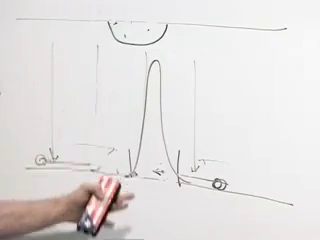
\includegraphics[width=0.82\textwidth]{lecture_05_figure_01.png}
\caption{第五次元の床と天井の描像。中心の地平面を伴う塊が、衝突後に床に沿って広がる。}
\lectureframe{00:04:22}
\end{figure}

地平面は永遠に残るわけではない。ホーキング放射がエネルギーを運び去り、四次元的な記述では、その放射は衝突から現れる通常のハドロンのシャワーである。検出器の事象における数千の飛跡は、この言葉では、双対ブラックホールから沸騰して出てくる粒子である。

\subsection{余分な次元は実在するのか。}

\begin{classroomqa}
\audiencequestion{第五の次元は空間的な次元であり、床と天井の間に描かれた線は文字通りその方向に延びているのか。}
\lecturerresponse{はい。それは空間的であり、その五次元幾何学に描かれた面は地平面である。余分な方向を``実在する''と呼ぶか、等価な数学的記述とみなすかは、より深い問いである。}
\end{classroomqa}

有用な主張は、重力が量子色力学を置き換えるということではない。むしろ、二つの言語が同じ物理を記述しうるということである。四次元的な言語では、通常の重力場を持たない、クォークとグルーオンの高温火の玉がある。五次元的な言語では、重力と地平面がある。対応が正しければ、正直なQCD計算と双対な重力計算は、両方が実行できるあらゆる場所で一致しなければならない。

\begin{classroomqa}
\audiencequestion{QCDには重力も地平面もない。ブラックホール描像は新しい物理を加えているのか、それとも単に火の玉を別の仕方で記述し直しているだけなのか。}
\lecturerresponse{四次元ではそれはクォークとグルーオンのプラズマであり、五次元的な姿では地平面を伴う重力による記述を持つ。利点は計算にある。強結合QCDは極めて難しいが、いくつかの地平面の性質---特に粘性---は比較的容易に計算できる。}
\end{classroomqa}

``実在の次元''と``数学的類推''の区別は、その記述が有用であるためにあらかじめ決着させる必要はない。ある構造は、他の変数とともに、より単純でより首尾一貫した法則の集合へと統合されるときに、物理的解釈を得る。とはいえ、事態を過大に述べるべきではない。観測されたクォーク--グルーオン・プラズマへのゲージ／重力双対性の応用は、強結合ダイナミクスの模型であって、現実世界のQCDが既知の厳密な重力双対をもつことの証明ではない。\editorialnote{この限定は、QCD応用の現代的な位置づけを明示するものであり、ここで展開した五次元の機構を変えるものではない。}

\section{なぜ衝突型加速器はビームを衝突させるのか}

ここで問いは実際的になる。なぜ単一のビームと静止標的ではなく、二つの運動するビームを用いるのか。なぜ円形加速器はそれほど大きいのか。なぜ電子と陽子は異なる扱いを受けるのか。これらの問いはすべて、相対論的エネルギーに関する問いである。

\begin{classroomqa}
\audiencequestion{なぜ一つの高エネルギー・ビームを静止標的に当てるのではなく、二つのビームを衝突させるのか。}
\lecturerresponse{新しい粒子を生み出すのは、重心系で利用可能なエネルギーである。等しく逆向きの二つの相対論的ビームは正味の運動量をもたないので、そのエネルギーの本質的にすべてが衝突に利用できる。固定標的では、入射エネルギーの多くが重心の運動として残ることを強いられる。}
\end{classroomqa}

大きさ\(p\)の逆向きの運動量をもつ二つの超相対論的粒子について、\(c=1\)単位での講義レベルの見積もりは
\begin{equation}
E_{\mathrm{cm}}^{\mathrm{collider}}\simeq 2p.
\end{equation}
である。対応する固定標的の見積もりは、ビーム運動量の平方根としてのみ増大する。
\begin{equation}
E_{\mathrm{cm}}^{\mathrm{fixed}}\sim \sqrt{mp}.
\end{equation}
重要なのは、省略された数因子ではなく、このスケーリングである。ビームエネルギーを二倍にすると衝突型加速器のエネルギーは二倍になるが、固定標的の重心エネルギーは平方根の分だけしか増加しない。

不変量の計算はこの比較を精密にする。\(P_1\)と\(P_2\)が入射四元運動量であるならば、
\begin{equation}
s=(P_1+P_2)^2,
\qquad E_{\mathrm{cm}}=\sqrt{s}.
\end{equation}
である。エネルギー\(E\)の等しい逆向きビームでは、空間的運動量が相殺し、\(\sqrt{s}=2E\)となる。エネルギー\(E\gg m\)の入射粒子が静止した等質量の標的に当たる場合、
\begin{equation}
s=2m^2+2mE,
\qquad
\sqrt{s}\simeq \sqrt{2mE}
\qquad (c=1).
\end{equation}
である。この短い不変量による導出は、口頭の見積もりで省略された因子を与える。\editorialnote{この導出は、講義のスケーリングの議論を再現可能にするために含められている。}

\begin{classroomqa}
\audiencequestion{円形加速器がこれほど大きくなくてはならない根本的な理由はあるのだろうか。同じビームを、より小さな装置の中でもっと何度も周回させることはできないのだろうか。}
\lecturerresponse{場と物質が限界を課す。粒子がメートルあたりに受け取るエネルギー増加は有限であるため、より高エネルギーの装置にはより大きな実効加速長が必要となる。また、きつい円はより大きな横方向の加速度を要求し、加速された電荷は放射する。リングが小さすぎれば、ビームは装置が供給するのと同じ速さでエネルギーを放射してしまう。}
\end{classroomqa}

曲げの関係は近似的に
\begin{equation}
p=qBR,
\end{equation}
である。したがって、磁場\(B\)を固定すれば、より大きな運動量\(p\)にはより大きな半径\(R\)が必要である。高周波空洞がビームエネルギーを高める仕事を行い、磁石がビームを曲げて集束する。広い教訓は黒板で与えられたもののままである。すなわち、場の強さと放射損失のため、任意に高エネルギーの加速器を小さなリングに圧縮することはできない。

円運動は、速さが一定でも速度が向きを変えるため加速度をもつ。加速された電荷はシンクロトロン放射を放出する。線形加速器は連続的な曲げによる損失を避けるが、短い加速の押し自体が文字通り放射を伴わないわけではない。円形機械は、同じ装置を各周回で再利用することと引き換えに、曲げのコストを受け入れる。

\begin{classroomqa}
\audiencequestion{なぜ電子はSLACの直線機械と結びつけられ、一方で円形高エネルギー衝突型加速器は陽子や他のハドロンを用いるのか。}
\lecturerresponse{電子ははるかに軽い。与えられた高エネルギーでは、そのローレンツ因子ははるかに大きく、円運動の加速度は電子をはるかに強く放射させる。より重い陽子は、シンクロトロン損失が手に負えなくなる前に、繰り返し周回して各周回でエネルギーを獲得できる。}
\end{classroomqa}

固定されたエネルギーとリング半径に対して、放射されるパワーは粒子質量とともに非常に急峻にスケールする。
\begin{equation}
P_{\mathrm{sync}}\propto \frac{E^4}{m^4R^2}.
\end{equation}
これが、電子--陽子の区別が、``軽い粒子の方が速く動く''という言葉が示唆するよりもはるかに鋭い理由である。両方のビームはすでに\(c\)に極めて近づき得るが、それらのローレンツ因子と放射損失は大きく異なる。\editorialnote{曲げの関係とシンクロトロンのスケーリングは、講義の定性的な加速器の議論を精密にする。それらは黒板では導出されなかった。}

\begin{classroomqa}
\audiencequestion{なぜハドロンも直線で加速しないのか。}
\lecturerresponse{それは可能である。困難は長さである。リングでは同じ粒子が加速構造を何度も通過する。等価な線形ハドロン機械は途方もなく長くなければならない。有用な妥協は大きなリングであり、陽子放射が許容できる程度に十分大きい。}
\end{classroomqa}

これらの加速器の問いは、ニュートンの規則がなぜ不十分であるかをまさに明らかにする。ここで特殊相対性理論に戻り、そのような比較を体系的にする言語を構築する。

\section{ガレージとリムジン}

約12フィートの長さのガレージと約20フィートの長さのストレッチリムジンを考える。運転手はリムジンがローレンツ収縮するまで加速し、それが収まることを期待する。ガレージの系では動いているリムジンは短いので、可能に見える。しかしリムジンの系では動いているガレージが短いので、不可能に見える。リムジン全体がガレージの中に入ることができるか。

壁との衝突が我々の注意をそらさないように、両方の扉を開ける。リムジンが中にあると言うことは、その前端と後端が\emph{同時に}中にあることを意味する。その最後の言葉にパズルのすべてが含まれている。

\(t\)を縦軸、\(x\)を横軸として時空図を描く。光線は\(c=1\)単位で\(45^\circ\)の光円錐を形成する。ガレージは静止しているので、その二つの扉の世界線は垂直である。リムジンの前端と後端は二本の平行な傾斜した世界線を描く。動いている系の\(t'\)軸は光円錐の方向に傾き、その同時線は傾いた\(x'\)軸に平行である。

\begin{figure}[H]
\centering
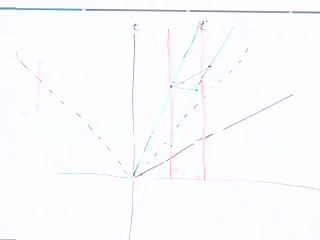
\includegraphics[width=0.82\textwidth]{lecture_05_figure_02.png}
\caption{完成したガレージ--リムジン時空図。垂直線がガレージを囲み、傾斜線がリムジンの両端を描く。水平および傾斜した切断は、二つの系の異なる同時スライスを表す。}
\lectureframe{00:31:05}
\end{figure}

ガレージの系では、水平線が二つのガレージ世界線の間で両方のリムジン世界線を横切ることができる。そのガレージ時刻では、後端は入っており、前端はまだ出ていない。収縮したリムジンは完全に中にある。

リムジンの系では、関連する同時事象は傾斜した線上にある。後端が入る事象を通るそのような線を描く。それは前端がすでに遠い扉を通過した後に前端世界線と交わる。リムジンはそれ自身の同時性によれば決して完全に中にはない。両方の主張は、異なる事象の対を比較しているので真である。

\begin{classroomqa}
\audiencequestion{二本の緑の世界線とそれらの間の水平線分は平行四辺形を形成するか。その黒い線分は車両の長さか。}
\lecturerresponse{水平線分はローレンツ収縮した長さである。なぜならその端点はガレージの系で同時だからである。固有長はリムジンの系で同時な端点から、\(x'\)に平行な線上で得られる。二つの測定は同じ世界線の対を通る異なる切断を用いる。}
\end{classroomqa}

\(L_0\)が固有長なら、水平なガレージ系の切断は長さ
\begin{equation}
L=\frac{L_0}{\gamma},
\qquad
\gamma=\frac{1}{\sqrt{1-v^2/c^2}}.
\end{equation}
を持つ。式だけではパラドックスを解決しない。図が解決する。なぜならどの事象が比較されたかを示すからである。相対性理論のパズルが二つの両立しない答えを生むように見えるときはいつでも、``同時に''の暗黙の使用を探せ。

\section{四つの座標と二つの添字位置}

パズルから運動法則へ移るために、幾何学を記憶する記法が必要である。座標を
\begin{equation}
(X^1,X^2,X^3,X^0)=(x,y,z,t),
\qquad X^\mu=(x,y,z,t),
\end{equation}
としてまとめる。ここで\(\mu\)は\(1,2,3,0\)を走る。この順序は、その添字が\(0\)であっても時間をページの最後に置き、黒板で用いられた慣習に一致する。

\begin{classroomqa}
\audiencequestion{我々は\(c=1\)と設定しているのか。通常の単位を復元すれば、時間座標は\(ct\)であるべきか。}
\lecturerresponse{はい。幾何学を展開する間は\(c=1\)と設定し、次元や非相対論的極限が問題になるときに\(c\)の因子を戻す。従来の長さの単位では、時間座標は\(ct\)である。}
\end{classroomqa}

同じベクトルは下付き添字で書くこともできる。ここで用いる符号の規約では、
\begin{equation}
X_\mu=(-x,-y,-z,t).
\end{equation}
したがって、添字を下げると3つの空間成分の符号が反転し、時間成分は変わらない。例えば、
\begin{equation}
X^\mu=(3,2,4,10)
\quad\Longrightarrow\quad
X_\mu=(-3,-2,-4,10).
\end{equation}
これらは2つの時空点ではなく、1つの幾何学的対象の2つの成分表示である。

\begin{classroomqa}
\audiencequestion{どの成分が共変でどれが反変か、また添字は上付きと下付きのどちらを意味するのか。}
\lecturerresponse{上付き添字の成分は反変であり、下付き添字の成分は共変である。教室で役立つ記憶法は``coは下、contraは上''である。物理学者はしばしば単に「上」と「下」と言う。}
\end{classroomqa}

この記法は不変な縮約
\begin{equation}
X_\mu X^\mu=t^2-x^2-y^2-z^2.
\label{eq:l5-interval}
\end{equation}
においてその価値を発揮する。微分形式ではこれは
\begin{equation}
d\tau^2=dt^2-dx^2-dy^2-dz^2
\qquad (c=1).
\label{eq:l5-proper-time}
\end{equation}
である。時間的運動では、\(d\tau\)は世界線に沿って動く時計が記録する時間である。

同じ添字が上に1回、下に1回現れるときはいつでも、和をとるものと理解される。アインシュタインの規約により
\begin{equation}
\sum_{\mu}X_\mu X^\mu
\end{equation}
は式~\eqref{eq:l5-interval}のより短い表現になる。これは単に活字上の節約ではない。ミンコフスキー幾何学の交代する符号が、あらゆる式で手作業で書き直されるのを防ぐのである。

\begin{classroomqa}
\audiencequestion{\(\tau\)は固有時間の標準的な記号か。}
\lecturerresponse{はい。記号\(s\)も使われることがあるが、\(\tau\)は固有時間の標準的な選択である。}
\end{classroomqa}

\section{容易な対称性としての回転}

ローレンツブーストは空間と時間を混ぜ合わせる。その行列を調べる前に、より馴染み深い空間軸の回転という操作を考えよう。相対運動が任意の方向を向いているなら、その方向が新しい\(x\)軸になるまで軸を回転させ、それから既知のブーストを適用すればよい。したがって回転は構成の一部であり、装飾的な回り道ではない。

\(z\)軸のまわりの角度\(\theta\)の回転では、
\begin{align}
x'&=x\cos\theta+y\sin\theta,\nonumber\\
y'&=-x\sin\theta+y\cos\theta,\label{eq:l5-rotation}\\
z'&=z.\nonumber
\end{align}
\(\theta=0\)ではこれらの式は\(x'=x\)と\(y'=y\)を与え、\(\theta=\pi/2\)では期待される符号で軸を交換する。

この変換はユークリッド距離を保つ。
\(c_\theta=\cos\theta\)および\(s_\theta=\sin\theta\)と書くと、
\begin{align}
x'^2+y'^2
&=(xc_\theta+ys_\theta)^2+(-xs_\theta+yc_\theta)^2\nonumber\\
&=x^2(c_\theta^2+s_\theta^2)
  +y^2(s_\theta^2+c_\theta^2)\nonumber\\
&\quad+2xyc_\theta s_\theta-2xyc_\theta s_\theta\nonumber\\
&=x^2+y^2.
\end{align}
交差項は相殺され、\(c_\theta^2+s_\theta^2=1\)となる。\(z'=z\)であるから、全長\(x^2+y^2+z^2\)は不変である。

同じ式は1つの行列方程式になる：
\begin{equation}
\begin{pmatrix}x'\\y'\\z'\end{pmatrix}
=
\underbrace{\begin{pmatrix}
\cos\theta&\sin\theta&0\\
-\sin\theta&\cos\theta&0\\
0&0&1
\end{pmatrix}}_{M}
\begin{pmatrix}x\\y\\z\end{pmatrix}.
\label{eq:l5-rotation-matrix}
\end{equation}
添字記法では、
\begin{equation}
x'^i=M^i{}_{j}x^j,
\qquad i,j=1,2,3.
\end{equation}

\begin{figure}[H]
\centering
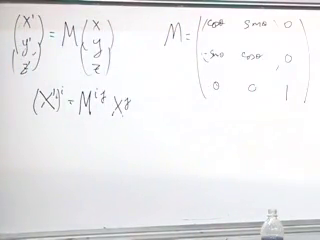
\includegraphics[width=0.82\textwidth]{lecture_05_figure_03.png}
\caption{行列方程式としても添字記法でも書かれた空間回転。}
\lectureframe{01:00:40}
\end{figure}

\section{ローレンツ行列と合成速度}

\(x\)に沿った運動について、\(c=1\)単位でのローレンツ変換は
\begin{align}
x'&=\gamma_v(x-vt), & y'&=y,\nonumber\\
z'&=z, & t'&=\gamma_v(t-vx),
\end{align}
ここで
\begin{equation}
\gamma_v=\frac{1}{\sqrt{1-v^2}}.
\end{equation}
成分の順序を\((x,y,z,t)\)とすると、これは
\begin{equation}
\begin{pmatrix}x'\\y'\\z'\\t'\end{pmatrix}
=
\begin{pmatrix}
\gamma_v&0&0&-\gamma_vv\\
0&1&0&0\\
0&0&1&0\\
-\gamma_vv&0&0&\gamma_v
\end{pmatrix}
\begin{pmatrix}x\\y\\z\\t\end{pmatrix}.
\label{eq:l5-lorentz-matrix}
\end{equation}
となる。

\begin{figure}[H]
\centering
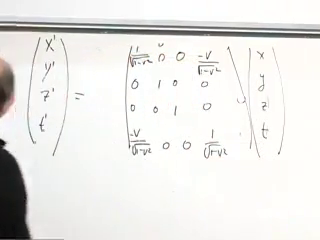
\includegraphics[width=0.82\textwidth]{lecture_05_figure_04.png}
\caption{\(4\times4\)ローレンツ行列。\(x\)成分と\(t\)成分だけが混ざり合い、\(y\)と\(z\)は変わらない。}
\lectureframe{01:04:40}
\end{figure}

行列の積が今や物理的な問いに答える。ある観測者が我々に対して速度\(v\)で運動し、第三の観測者がその観測者に対して速度\(u\)で運動しており、すべて同じ軸に沿っているとしよう。ニュートン力学の運動学では\(w=u+v\)を与え、それでは\(3c/4\)の2つの速度が合成されて\(3c/2\)になることが許されてしまう。相対性理論は異なる規則を与えなければならない。

ブーストの実質的な部分は\(2\times2\)行列
\begin{equation}
B(v)=\gamma_v
\begin{pmatrix}1&-v\\-v&1\end{pmatrix}.
\end{equation}
である。2つのブーストを合成すると
\begin{align}
B(u)B(v)
&=\gamma_u\gamma_v
\begin{pmatrix}1&-u\\-u&1\end{pmatrix}
\begin{pmatrix}1&-v\\-v&1\end{pmatrix}\nonumber\\
&=\gamma_u\gamma_v
\begin{pmatrix}
1+uv&-(u+v)\\
-(u+v)&1+uv
\end{pmatrix}.
\label{eq:l5-composed-boost}
\end{align}
非対角成分と対角成分の比が、結果として得られるブーストの速度を特定する：
\begin{equation}
w=\frac{u+v}{1+uv}
\qquad(c=1).
\end{equation}
次元を復元すると、
\begin{equation}
w=\frac{u+v}{1+uv/c^2}.
\label{eq:l5-velocity-addition}
\end{equation}

\begin{figure}[H]
\centering
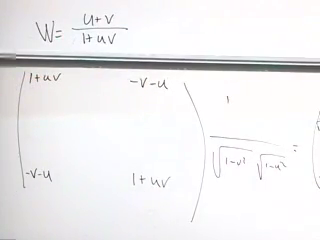
\includegraphics[width=0.82\textwidth]{lecture_05_figure_05.png}
\caption{合成ブースト行列と自然単位での速度
\(w=(u+v)/(1+uv)\)。}
\lectureframe{01:15:35}
\end{figure}

\(u\)と\(v\)がそれぞれ\(c\)に近いなら、分子は\(2c\)に近づき、分母は\(2\)に近づくので、\(w\)は\(2c\)ではなく\(c\)に近づく。より一般には、式~\eqref{eq:l5-velocity-addition}は光速以下の入力を光速以下の結果に写す。行列の積が速度限界を自動的に組み込んでいるのである。

\section{4元ベクトルと通常の速度の破綻}

4元ベクトルとは、その4つの成分が時空座標と同じように回転とローレンツブーストの下で変換するような対象である。\(V^\mu\)が4元ベクトルなら、ここでの符号の規約では
\begin{equation}
V_\mu=(-V^1,-V^2,-V^3,V^0),
\end{equation}
であり、その不変ノルムは
\begin{equation}
V_\mu V^\mu=(V^0)^2-(V^1)^2-(V^2)^2-(V^3)^2.
\end{equation}
である。2つの4元ベクトル\(V^\mu\)と\(W^\mu\)について、縮約
\begin{equation}
W_\mu V^\mu
=W^0V^0-W^1V^1-W^2V^2-W^3V^3
\end{equation}
も同様に不変である。成分は座標系の間で変化するが、縮約は変化しない。

通常の速度は3つの成分しか持たない。
\begin{equation}
\mathbf v=\left(\frac{dx}{dt},\frac{dy}{dt},\frac{dz}{dt}\right).
\end{equation}
\(dt/dt=1\)を付け加えても、それは有用な4元ベクトルにはならない。第4成分は自明なものになり、得られる対象はローレンツ変換の下で線形に変換されない。座標時間\(t\)は慣性系ごとに変わるので、\(t\)で微分すると望ましい変換則が損なわれる。

固有時間がその解決を与える。世界線に沿って
\begin{equation}
u^\mu=\frac{dX^\mu}{d\tau}.
\label{eq:l5-four-velocity}
\end{equation}
と定義する。微分\(dX^\mu\)は4元ベクトルであり、\(d\tau\)は不変量であるから、その比は4元ベクトルである。``固有''という形容詞は分母にある時計を指す。

連鎖律により、この対象は通常の速度と関係づけられる：
\begin{equation}
\frac{dx}{d\tau}=\frac{dx}{dt}\frac{dt}{d\tau},
\end{equation}
であり、\(y\)および\(z\)についても同様である。式~\eqref{eq:l5-proper-time}より
\begin{align}
\left(\frac{d\tau}{dt}\right)^2
&=1-\left(\frac{dx}{dt}\right)^2
    -\left(\frac{dy}{dt}\right)^2
    -\left(\frac{dz}{dt}\right)^2\nonumber\\
&=1-v^2
\qquad(c=1),
\end{align}
したがって
\begin{equation}
\frac{dt}{d\tau}=\gamma_v=\frac{1}{\sqrt{1-v^2}}.
\end{equation}
4つの成分は
\begin{equation}
u^i=\gamma_v v^i,
\qquad
u^0=\gamma_v
\qquad(c=1).
\label{eq:l5-four-velocity-components}
\end{equation}
である。低速では\(u^i\simeq v^i\)および\(u^0\simeq1\)である。光速に近づくと、\(\gamma_v\)は際限なく増大し、固有速度は通常の速度と著しく異なる。

\begin{figure}[H]
\centering
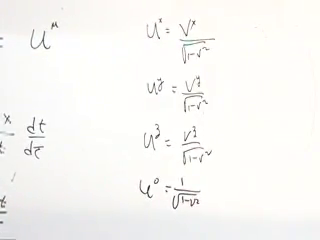
\includegraphics[width=0.82\textwidth]{lecture_05_figure_06.png}
\caption{通常の速度とローレンツ因子によって表された固有速度の4成分。}
\lectureframe{01:34:40}
\end{figure}

従来の単位を復元し、\(X^0=ct\)を用いると、ここで採用している空間成分を先に置く順序で標準的な形
\begin{equation}
U^\mu=(\gamma_v\mathbf v,\gamma_v c)
\end{equation}
が得られる。その不変ノルムは
\begin{equation}
U_\mu U^\mu=c^2.
\end{equation}
である。したがって、すべての質量を持つ粒子は、その空間速度が慣性系に依存しても、同じ不変的大きさの4元速度を持つ。

\section{世界線の接線}

式~\eqref{eq:l5-four-velocity}には、よく知られたユークリッド的な模型がある。通常の3次元空間内の曲線に沿って
\begin{equation}
ds^2=dx^2+dy^2+dz^2.
\end{equation}
である。微分変位\((dx,dy,dz)\)は曲線に沿う方向を向くが、単位ベクトルではない。弧長で割ると
\begin{equation}
\mathbf T=
\left(\frac{dx}{ds},\frac{dy}{ds},\frac{dz}{ds}\right),
\qquad
\mathbf T\cdot\mathbf T=1.
\end{equation}
が得られる。相対論的な構成は、ユークリッド的弧長の代わりに固有時間を用いた同じ考え方である。ベクトル\(u^\mu=dX^\mu/d\tau\)は世界線に接している。

\begin{figure}[H]
\centering
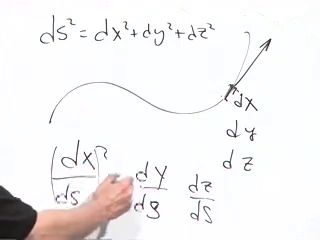
\includegraphics[width=0.82\textwidth]{lecture_05_figure_07.png}
\caption{ユークリッド的な接ベクトルの構成：微分変位を弧長要素\(ds\)で割る。固有時間は時間的向きの世界線に沿って同様の役割を果たす。}
\lectureframe{01:39:30}
\end{figure}

\begin{classroomqa}
\audiencequestion{もし\(c=1\)ならば、固有時間と固有距離は同じものか。}
\lecturerresponse{\(c=1\)と置くと時間と距離が同じ単位になるが、時空幾何学の負号が消えるわけではない。ユークリッド的な類推では、\(s\)は空間的曲線に沿って測った通常の距離である。時間的向きの世界線に沿っては、\(\tau\)は時計によって測られた経過時間である。構成は類似しているが、幾何学は異なる。}
\end{classroomqa}

もう一度微分すると固有加速度が定義される：
\begin{equation}
a^\mu=\frac{du^\mu}{d\tau}.
\end{equation}
これは、ニュートンの第2法則を相対論的にする際に\(d^2\mathbf x/dt^2\)を置き換えなければならない量である。\(u_\mu u^\mu\)は定数であるから、
\begin{equation}
\frac{d}{d\tau}(u_\mu u^\mu)=2u_\mu a^\mu=0,
\end{equation}
であり、したがって4元加速度は4元速度とミンコフスキー直交する。\editorialnote{この直交性は不変ノルムから直ちに従い、定義の次に来る数学的帰結として含められている。}

\section{4元運動量とエネルギー}

運動量を最後の例とするのは、それが衝突や崩壊において保存されるからである。粒子は固定された固有質量\(m\)を持ち、これはしばしば静止質量と呼ばれる。それは速度によって変化しない。相対論的運動量は、その固定された質量と4元速度の積である：
\begin{equation}
p^\mu=mu^\mu.
\label{eq:l5-four-momentum}
\end{equation}
\(c=1\)単位では
\begin{equation}
p^i=\gamma_v m v^i,
\qquad
p^0=\gamma_v m.
\end{equation}
である。小さな速度では\(\gamma_v\simeq1\)であるから、空間成分はニュートン的な運動量\(m\mathbf v\)に帰着する。高速ではそれらは\(m\mathbf v\)よりも急速に増大する。

時間成分はエネルギーである。従来の単位と\(X^0=ct\)を用いると
\begin{equation}
P^\mu=(\mathbf p,E/c)
=(\gamma_v m\mathbf v,\gamma_v mc),
\end{equation}
であり、したがって
\begin{equation}
E=\gamma_v mc^2
=mc^2\left(1-\frac{v^2}{c^2}\right)^{-1/2}.
\label{eq:l5-relativistic-energy}
\end{equation}
である。

通常の力学を回復するために、
\(\epsilon=v^2/c^2\ll1\)とおく。二項展開により
\begin{equation}
(1-\epsilon)^p=1-p\epsilon+O(\epsilon^2).
\end{equation}
が得られる。\(p=-1/2\)ととると、
\begin{align}
E
&=mc^2\left(1-\frac{v^2}{c^2}\right)^{-1/2}\nonumber\\
&=mc^2\left[1+\frac12\frac{v^2}{c^2}
  +O\!\left(\frac{v^4}{c^4}\right)\right]\nonumber\\
&=mc^2+\frac12mv^2+O\!\left(\frac{mv^4}{c^2}\right).
\label{eq:l5-energy-expansion}
\end{align}

\begin{figure}[H]
\centering
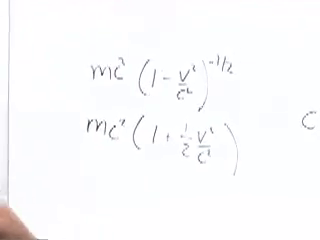
\includegraphics[width=0.82\textwidth]{lecture_05_figure_08.png}
\caption{相対論的エネルギーの低速展開。静止エネルギーとニュートン的運動エネルギーが現れる。}
\lectureframe{01:51:30}
\end{figure}

最初の項\(mc^2\)は、静止していても存在する。質量が変化しない固定された粒子の集まりを扱うニュートン的な問題では、その項は運動の前後で同じ定数を加えるだけなので、よく知られた収支に影響するのは\(\tfrac12mv^2\)だけである。相対論は、捨てられていたその定数が実はずっと物理的なエネルギーであったことを明らかにする。

したがって、エネルギーと運動量は無関係な保存則ではない。それらは1つの保存ベクトルの4つの成分である。ローレンツブーストはそれらを混合する：ある観測者がエネルギーと呼ぶものは、別の観測者の運動量に部分的に寄与し、その逆も成り立つ。それにもかかわらず、孤立系では、全4元運動量はすべての慣性系においてあらゆる衝突や崩壊の前後で同じである。

ここが相対論的力学の閾値である。次の課題は、力を固有加速度によって表すこと、および相対論的波動方程式、とりわけ電磁気学と光を支配する方程式を理解することである。